\documentclass[sigconf]{acmart}

\usepackage{booktabs} % For formal tables
\usepackage{array,multirow}
% Copyright
%\setcopyright{none}
%\setcopyright{acmcopyright}
%\setcopyright{acmlicensed}
\setcopyright{rightsretained}
%\setcopyright{usgov}
%\setcopyright{usgovmixed}
%\setcopyright{cagov}
%\setcopyright{cagovmixed}
%\usepackage{setspace}
\pagestyle{empty} 
%\doublespacing

% DOI
\acmDOI{10.475/123_4}

% ISBN
\acmISBN{123-4567-24-567/08/06}

%Conference
%\acmConference[WOODSTOCK'97]{ACM Woodstock conference}{July 1997}{El Paso, Texas USA} 
%\acmYear{1997}
%\copyrightyear{2016}


%\acmArticle{4}
%\acmPrice{15.00}

% These commands are optional
%\acmBooktitle{Transactions of the ACM Woodstock conference}
%\editor{Jennifer B. Sartor}
%\editor{Theo D'Hondt}
%\editor{Wolfgang De Meuter}


\begin{document}
%\title{Detecting Emergency Situations Based on Locations in Twitter}
%\title{Detecting Emergency Situations in Twitter Using Self-Organized Citizen Sensors}
\title{Domain-Independent Detection of Emergency Situations\\Based on Social Activity Related to Geolocations}

%\titlenote{Produces the permission block, and
 % copyright information}
 
 
%\subtitle{Extended Abstract}
%\subtitlenote{The full version of the author's guide is available as
  %\texttt{acmart.pdf} document}


\author{Hernan Sarmiento}
%\authornote{Dr.~Trovato insisted his name be first.}
%\orcid{1234-5678-9012}
\affiliation{%
  \institution{Department of Computer Science, University of Chile}
  \streetaddress{P.O. Box 1212}
   \city{Santiago} 
   \country{Chile}}
\email{hsarmien@dcc.uchile.cl}

\author{Barbara Poblete}
%\authornote{The secretary disavows any knowledge of this author's actions.}
\affiliation{%
  \institution{Department of Computer Science, University of Chile}
  \streetaddress{P.O. Box 1212}
   \city{Santiago} 
   \country{Chile}}
\email{bpoblete@dcc.uchile.cl}

\author{Sergio Campos}
%\authornote{This author is the
 % one who did all the really hard work.}
\affiliation{%
  \institution{Department of Geophysics, University of Chile}
%  \streetaddress{1 Th{\o}rv{\"a}ld Circle}
  \city{Santiago} 
  \country{Chile}}
\email{jaime@dgf.uchile.cl}



% The default list of authors is too long for headers.
%\renewcommand{\shortauthors}{B. Trovato et al.}


\begin{abstract}
%Most methods to detect emergency situations using Twitter rely on keyword. The problem of keyword-based methods is the need to train in specific domains and language for different type of events, for example: earthquakes, typhoons, terrorist attacks, tornadoes, etc. Our proposal is to rather use the recurring mention of a country locations in microblogging messages to identify such events without using keywords and characterize through of interarrival time probability distributions. Our method use a SVM classifier that is independent of the text language of the messages and can be training and testing among different languages and domains.
%
Most methods for detecting emergency situations using Twitter rely on identifying features within messages that contain domain-specific keywords. However, keyword-based methods require models to be trained on historical data of specific domains, in multiple languages, and for different types of events (e.g., earthquakes, floods, wildfires, etc.). 
%
In addition to being costly, these approaches may fail to detect previously unexpected situations, such as uncommon catastrophes or terrorist attacks.
%
Nevertheless, collective mentions of keywords are not the only type of self-organizing phenomena that may arise when a real-world extreme situation occurs.
%
Just as physical sensors become activated when stimulated, localized citizen sensors will also react in a similar manner.  
%
To leverage this information, we propose to use self-organized geolocation related activity to identify emergency situations.
%
We propose to detect such events by tracking the frequencies, and probability distributions of the interarrival time of the messages related to specific locations.
%
Using an off-the-shelf classifier that is independent of domain-specific features, we study and describe emergency situations based solely on location-based features in messages.
%
Our findings indicate that anomalies in location-related social media user activity indeed provide information for automatically detecting emergency situations independent of their domain.
\end{abstract}




%
% The code below should be generated by the tool at
% http://dl.acm.org/ccs.cfm
% Please copy and paste the code instead of the example below. 
%
\begin{CCSXML}
	<ccs2012>
	<concept>
	<concept_id>10002951.10003227.10003351.10003446</concept_id>
	<concept_desc>Information systems~Data stream mining</concept_desc>
	<concept_significance>500</concept_significance>
	</concept>
	<concept>
	<concept_id>10002951.10003227.10003236</concept_id>
	<concept_desc>Information systems~Spatial-temporal systems</concept_desc>
	<concept_significance>300</concept_significance>
	</concept>
	</ccs2012>
\end{CCSXML}

\ccsdesc[500]{Information systems~Data stream mining}
\ccsdesc[300]{Information systems~Spatial-temporal systems}

\keywords{Emergency Situations, Citizen Sensors, Social Media}


\maketitle

\section{Introduction}
Social media has become a major communication channel during high-impact real-world events, such as elections, sports events, emergency situations, among others. In each case, users act as ``citizen sensors'' sharing and posting their mood, opinion, photos, videos and geographical points of interest.

During emergency situations, traditional media may suffer infrastructure issues and real-time communications could be disrupted. Instead, microblogging has played a critical role over the last fifteen years allowing users to share real-time information from people local to the incident, such as status updates, casualties, damages and alerts \cite{kumar2011tweettracker,imran2013extracting,stowe2016identifying,reuterfifteen}. For this reason, researchers have studied user behavior during these events to detect, summarise and classify messages with the goal of helping authorities, and the general public, with situational awareness to provide fast and conscientious responses during crisis situations.

Twitter is a microblogging platform that allows users to share short messages (called \textit{tweets}) and is currently used worldwide by over $300$ million people.\footnote{http://www.statista.com/statistics/282087/number-of-monthly-active-twitter-users/} About $80\%$ of Twitter users access from mobile devices, which contributes to the immediacy of diffusion of information, especially during crisis situations \cite{castillo2016big}. One of the most important tasks during these situations, is to timely detect incoming real-world events. This is because, as with most social media conversations, messages are often overridden with irrelevant and redundant noise. In current works \cite{kumar2011tweettracker,caragea2011classifying,imranaidr2014,maldonado2017}, these tasks are solved with methods that rely on keyword based filters on the \textit{Twitter Public Streaming API}.\footnote{https://developer.twitter.com/en/docs/tweets/filter-realtime/overview} The problem with keyword-based methods is the need to train in specific domains for different type of events. For instance, \citeauthor{olteanu2014} \cite{olteanu2014} generate a set of keywords based on different datasets. However, this is not sufficient for cases in which specific and previously unseen terms arise for a particular event (e.g., \textit{\#eqnz} for Earthquakes in New Zealand, or \textit{\#pabloph} for Typhoon Pablo in Philippines) \cite{potts2011tweeting,bruns2012local,karimi2013classifying}. Furthermore, these sets of keywords are commonly obtained a particular language and will not work in others.

Additionally, several works related to crisis situations show a strong relationship between a type of event (what) and the spatiotemporal dimensions (when and where). For example, it has been observed that top trends during earthquakes are related to location mentions \cite{mendoza2010twitter}, also, that there is a strong relationship between the proximity to a hurricane path and hurricane-related social media activity \cite{kryvasheyeu2016rapid}. Other works have addressed the extraction of locations and points of interest during floods \cite{lingad2013location}, as well as mixing geographic information system (GIS) information with geo-tagged messages to improve disaster mapping and real-time event tracking \cite{huang2015disastermapper}.

Based on previous works, the question we address here is: \textit{Is there evidence to detect an emergency situation based on anomalies in messages related to contain locations?}.

Here, we propose a method based on recurring references to country level locations in message metadata. For this task, we create a gazetteer tree based on the hierarchy of the specific country, divide the messages into fixed time-windows and compute the frequency and the probability distributions of the interarrival time of the messages for each geographical hierarchy. To detect an emergency situation, we train a SVM classifier by each hierarchy and apply a geographic spread to filter false positives detection considering that an emergency situation can be \textit{Focalized} or \textit{Diffused}.  

Our main contribution is to create a methodology that detects instantaneous emergency situations just by using the location related information for a specific country. Furthermore, our classifiers do not depend on language to detect a new event since they do not use textual features as input. Moreover, we characterize crisis situations that affect small or large geographical areas.

The paper is organized as follows: we first introduce an overview of relevant literature related to emergency situation and event detection in social media. Next we present a complete description of our proposal divide in four parts. Thereafter, we provide a full description of our dataset and later we summarise our experimental validation over the ground truth and on-line evaluation. Finally, we deliver our discussions, conclusions and future work.



\section{Related Work}

We discuss relevant work for our proposal, primary from two areas: (1) crisis-related social media monitoring and (2) event detection based on locations.

\subsection{Crisis-Related Social Media Monitoring}

Twitter has been used extensively during emergency situations to extract and identify relevant information. However, social media communications during emergency situations have become so abundant that it is necessary to sift through millions of data points to find information that is most useful during a given event \cite{imran2015processing}.

One of the main tasks related to emergency situations is to detect a new real-crisis event in social media. Most existing event-detection methods described in the literature are based on keywords. For instance, \textit{TweetTracker} \cite{kumar2011tweettracker} presented a case study using tweets that discuss a cholera outbreak in Haiti. The primary mechanism for monitoring tweets is through specific keywords and hashtags filters related to the Haiti. To detect a new event, emerging trends are identified based on the analysis of older tweets. In the same way, \textit{EMERSE} \cite{caragea2011classifying} used a set of keywords related to the Haiti earthquake and applies a random forests algorithm for classifying messages. Likewise, the \textit{Twicalli} system \cite{maldonado2017} introduced an unsupervised approach to detect earthquakes that only requires a general list of keywords. 

Researchers at CSIRO Australia proposed \textit{ESA} \cite{cameron2012emergency,yin2012esa}, a system to detect disasters in Australia and New Zealand. This system is based on a probabilistic method to identify bursty keywords and historical data to build a language model of word occurrences. Alerts are identified if a term has a probability distribution that significantly deviates from the language model. Similarly, \textit{Twitcident} \cite{abel2012twitcident} system was developed for detecting incidents which relies on emergency broadcasting services, such as the police, the fire department and other public emergency services. The \textit{Twitcident} framework translates the broadcasted message into an initial incident profile that is applied as query to collect messages from Twitter, where an incident profile is a set of weighted attribute-value pairs that describe the characteristics related to the incident. 

\textit{CrisisLex} \cite{olteanu2014} is introduced to extract different crisis-related terms to filter messages in Twitter. In this work,
authors collected six disasters which affected several millions of people. Data was collected from Twitter using two samples: a keyword-based sample and location-based sample. Based on datasets, they created a lexicon of the most frequent terms that appear in relevant messages posted during different types of crisis situations.

Our current work, on the other hand, is based on detecting events by monitoring \textit{zscore} variations through fixed time-windows.

\subsection{Event Detection Based on Locations}

In addition to crisis-related social media monitoring, there are also some unsupervised event detection approaches based on location information. \textit{Jasmine} \cite{watanabe2011jasmine} detected local real-world events using geolocation information from microblog documents. To detect such events, they identify a group of tweets that describe a particular theme, which are generated within a short time frame and a same geographic area. Similarly, \citeauthor*{unankard2015emerging} \cite{unankard2015emerging} proposed an approach for early detection of emerging hotspot events in social networks with location sensivity. In this work, the authors identified strong correlations between user locations and event locations when detecting emerging events using content similarity between clusters. In the work of \citeauthor{walther2013geo} \cite{walther2013geo} real-world events were detected in a small scale with messages from the New York metropolitan area. There, clusters were created for each candidate event and evaluated using cluster score based on textual features (sentiment analysis, common theme, duplicate, etc) and other features (tweet count, unique coordinates, etc.).

Supervised approaches have also been proposed. \textit{TEDAS} \cite{li2012tedas} detected, analysed and identified events using refined rules (e.g., keywords, hashtags) and classify messages based on content as well Twitter specific features as URLs, hashtags and mentions. Besides, location information is extracted using both explicit geographical coordinates and implicit geographical references in the content. In the same way, \citeauthor{becker2011beyond} \cite{becker2011beyond} proposed an on-line clustering technique, which continuously clusters similar tweets and then classifies the clusters using Support Vector Machine algorithm. Finally, events (clusters) are classified into real-world events or nonevents.

\medskip

\noindent{\textbf{Summary.}} Most previous works to detect an emergency situations rely on keywords using probabilistic temporal models for specific domains (e.g., keywords or location). In general terms, these approaches need knowledge about the event and a new emerging topic referring to a crisis cannot be identified to detect an emergency situation. In the case of the works on event detection based on locations, they are designed to be applied in a small area and based on historical data. Regardless of which approach is implemented (supervised or unsupervised), textual features are the most used attributes to characterise an event and on-line clustering is the most common technique to create candidate events.

Based on the works presented by \citeauthor{guzman2013line} \cite{guzman2013line} and \citeauthor{maldonado2017} \cite{maldonado2017}, we extend the ideas of bursty keywords and \textit{z-score} variation between fixed time-windows and we apply these proposals over locations to identify anomalies in social media activity. Furthermore, we do not use a set of keywords to detect specific types of events (e.g., earthquake, flood or terrorist attack). In contrast, our proposal is focused on detecting such events by tracking frequencies, and probability distributions of the interarrival time of the messages related to specific locations.



\section{Proposed Approach}

In order to provide a complete coverage of location-based detection of emergency situations, we propose an approach which has four stages (depicted in the Data Process module in Figure \ref{fig:diagram}). Next, we describe each stage:

\begin{figure}
	\centering
	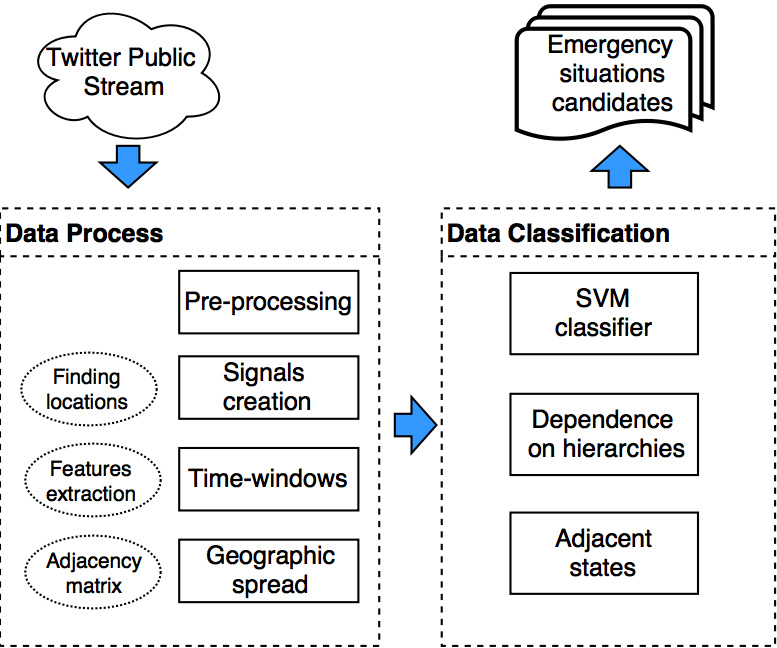
\includegraphics[width=\columnwidth]{img/diagram2.png}
	\caption{Key components of the proposed approach.}
	\label{fig:diagram}
\end{figure}

\subsection{Data Pre-Processing}
%In this stage, data is pre-processed from Twitter Streaming API\footnote{algo}, which allows access to subsets equal to $1\%$ of public status descriptions in real-time. With this tool, we can be retrieve messages using a set of keywords or messages from specific locations setting a bounding box. In our approach, we get entire subsets of messages without use keywords or specific locations. Then, we retrieve random messages about any topic and any place in the world.

%To increase the number of messages related to locations, we consider tweets and retweets messages. 
Since we consider users as citizen sensors, we filter messages depending of native language of each country using the attribute \textit{lang} retrieved from the metadata in tweets.\footnote{https://developer.twitter.com/en/docs/tweets/data-dictionary/overview/tweet-object} For example, if we analyse Italy, we just consider messages in Italian. Finally, we remove user mentions, URLs,  special characters and apply text tokenization. Also we do not remove hashtags or stopwords because some locations can be included in hashtags terms and some places can contain stopwords that can differentiate them from other similar non-related to locations terms.

\subsection{Signal Creation}
The problems that we address in this stage are how to infer locations from microblog messages to track signals over time in the data stream and what is the lowest hierarchy level to find and assign to these signals.

\subsubsection{Geographical Hierarchy}\label{sssec:geohie}
Using the idea of \textit{Gazetteer as a Tree} presented in \cite{yin2014pinpointing} in which each place is associated with a canonical taxonomy node, we construct our gazetteer tree based on Geonames\footnote{http://download.geonames.org/export/dump/} and Wikipedia\footnote{http://www.wikipedia.org/} for each country to analyse. However, in \cite{yin2014pinpointing} the gazetteer hierarchy presents four levels where the lowest level represents a specific point of interest. In our approach, we use a subset of the gazetteer hierarchy with three levels, in which the lowest level is represented by a city since a large amount of users specify their location down to this level \cite{hecht2011tweets}. For example, if we have the \textit{city:Manchester}, we associate this location with \textit{region-state:North West} and also with \textit{country:England}. Furthermore, the name of locations are considered just in the native language of the country. For instance, in the case of Italy locations, we consider \textit{Roma} and not \textit{Rome}.

\subsubsection{Finding Locations in Microblog Metadata}

The structure of the Tweet metadata obtains information about the message and the user who shares a message. Considering the geographical hierarchy explained in the previous section, we search these locations on different levels of metadata and create one signal for each as following:

\begin{itemize}
	\item Tweet Text: location is mentioned in the attribute \texttt{text} of tweet object, that is, on the body of the message.
	\item User Location: location is mentioned in the attribute \texttt{location} inside the \texttt{user object}, that is, the location set by the user in his profile.
	\item Tweet Text - User Location: location is mentioned in the attribute \texttt{text} of tweet object and also location is mentioned in the attribute \texttt{location} inside the \texttt{user object}. This means that the location is mentioned in the body of the message and the user who shares message has the same location in his profile. In this case, tweet text and user location can be different in the smallest hierarchy, but in the highest level can be equal. 
\end{itemize}

In this way, mixing geographical hierarchy and locations in microblog metadata, we create $NxM$ signals where $N$ is the number of locations obtained by gazetteer tree and $M$ is the number of metadata-levels extracted from Tweet Object. For instance, we create a signal for \textit{city:Manchester} and we find this hierarchy in \textit{metadata:Tweet Text} and also in \textit{metadata:User Location}. That means that we track the mention of \textit{city:Manchester} at the level of the body of message and at the level of the location of the user profile individually.

\subsection{Time-Windows}
In this stage we address the problems of how to divide and determine the time-window size to detect a new emergency situation and what features by the time-window allow it.

\subsubsection{Determining Optimal Window Size}

According to \citeauthor{guzman2013line} \cite{guzman2013line}: ``If the window size is too small, the ocurrence of empty windows for a term increases, making the noise rate increase and frequency rate tend towards zero. On the other hand, if the window size is too large, the stability of the signal becomes constant and bursty keyword detection is delayed''. Using this definition, we divide our signals into windows of six minutes because it divides a 24-hour day exactly, making the analysis easier to understand and to compare from different days.


\subsubsection{Normalized Frequency}
We compute the number of the messages of each time-window by signal. To normalize frequency, we compute \textit{z-score} as following:

\begin{equation} \label{eq:1}
zscore = \frac{x_{i} - \mu_{k} }{\sigma_{k}}
\end{equation}

where $x_{i}$ is the frequency of the current $i$ time-window, $\mu_{k}$ and  $\sigma_{k}$ are mean and standard deviation of the previous $k$ time-windows respectively.

%\begin{itemize}
%	\item We calculate the number of messages of each time windows for each signal.
%	\item In our first approach, we compute max-min normalization and z-score normalization of all time windows for each signal. This approach is wrong because we do not know the next values in the streaming. We just know the previous values.
%	\item We compute the z-score normalization using past values for each signal independently. We do not use rolling/moving z-score because some signals have Null values of frequency. It is happen in smallest cities or states.
%\end{itemize}
\subsubsection{Interarrival Time}

To characterize the urgency of the messages during a time-window, we use our previous results \cite{DBLP:conf/fdia/Sarmiento17} to compute the \textit{interarrival time} which is defined as $d_{i} = t_{i+1} - t_{i}$, where $d_{i}$ denotes the difference between two consecutive social media messages $i$ and $i+1$ that arrived in moments $t_{i}$ and $t_{i+1}$ respectively. Using this definition and according the work of \citeauthor{kalyanam2016prediction} \cite{kalyanam2016prediction}, high-activity events have a high-frequency in the first bins represented by values $d_{i} \approx 0$. 

To quantify a high-frequency in very small values of $d_{i}$, we compute the measures \textit{skewness} and \textit{kurtosis}, which represent the asymmetry and the tailedness of the shape of probability distribution respectively \cite{mardia1970measures}. Finally, we apply the equation \ref{eq:1} over \textit{skewness} and \textit{kurtosis} to calculate variation based on previous values.

%\begin{itemize}
%	\item Inter-arrival time represent the difference between 2 consecutive messages for one signal. In this case, a small difference between a set of messages represent the urgency or relevancy in a specific time (reference to plosone paper)
%	\item First, we compute inter-arrival time for each time windows independently. We summary results using quantiles, mean, min and max values. The problem with this approach is that we can not compare values between signals because each signal has different frequencies and behaviours along the time.
%	\item We compute skewness and kurtosis which represent a measure of the asymetry and "taildness" of the probability distribution respectively. In both case, we calculate the measures using previous values such as z-score normalization.
%\end{itemize}

%\subsection{Subsetting Signals}
%\begin{itemize}
%	\item Several signals have a null values along the time. For example, any city that is not a big city or capital city, does not a continuous frequency. To avoid this behaviour, we use cities just for compute the state frequency signal and later we discard them. Finally, we just monitor states and country hierarchy.
%	\item Furthermore, we remove gps signal because just 1-3 percent of messages have gps activated.
%\end{itemize}

\subsection{Geographic Spread}\label{sssec:geospread}

An emergency situation that affects and mobilizes response in a small area is defined as \textit{focalized}, while a disaster with a large geographic impact is defined as \textit{diffused} \cite{olteanu2015expect}. Using this definition, we extend this concept to represent neighborhoods between locations obtained from section \ref{sssec:geohie}. For that purpose, we create an \textit{adjancency matrix} $M$, where $M_{i,j} = 1$ represents if two locations are geographically connected and $M_{i,j} = 0$ if they are not connected. For instance, if an event is diffused (e.g., earthquake), the detection should be in adjacent-locations independentely of metadata-level. On the other hand, if an event is focalized (e.g., terrorist attack), just one location should be detected but in different metadata-levels simultaneously.


\begin{table}
	\caption{List of earthquakes studied as ground truth, sorted by date.}
	\label{tab:eqs}
	\begin{tabular}{lccl}
		\toprule
		Country&Datetime (UTC)&Magnitude (Mw)& Language\\
		\midrule
		Italy & 2016-10-26 17:10:36 & 5.5 & Italian \\
		Italy & 2016-10-30 06:40:17 & 6.6 & Italian\\
		Chile & 2016-12-25 14:22:26 & 7.6 & Spanish\\
		Chile & 2017-04-23 02:36:06 & 5.9 & Spanish\\
		Chile & 2017-04-24 21:38:28 & 6.9 & Spanish\\
		\midrule
		%\bottomrule
	\end{tabular}
\end{table}

\section{Dataset}

Data is collected from Twitter Public Streaming API, which allows access to subsets equal to $1\%$ of public status descriptions in real-time. With this tool, we can retrieve either messages using a set of keywords or messages from specific locations setting a bounding box. In our approach, we get entire subsets of messages without use keywords or specific locations. Then, we retrieve random messages about any topic and any place in the world.
 
\subsection{Ground Truth}

We analyse five earthquakes with magnitudes between $5.5Mw$ and $7.6Mw$\footnote{Mw: the moment magnitude scale}, ocurring in Italian-speaking and Spanish-speaking countries between October 2016 and April 2017 (Table \ref{tab:eqs}). For that purpose, we collect $20$ million of messages 12-hours before and after the emergency situation events. 

According our proposal we create both the gazetteer hierarchies\footnote{http://users.dcc.uchile.cl/$\sim$hsarmien/gazetteer.html} for each country and construct the signals based on each hierarchy and metadata-level. As a result of the number of messages of each signal (Table \ref{tab:message_signal}), we discard all signals related to city hierarchy since a great amount of small cities have zero frequency in a normal situation unlike to capital or metropolitan cities.




\begin{table}
	\caption{Number of messages by signal.}
	\label{tab:message_signal}
	\begin{tabular}{ccl}
		\toprule
		Hierarchy&Metadata-level&Messages\\
		\midrule
		All & All & 87,291 \\
		\midrule
	    \multirow{3}{*}{Country} & Tweet Text & 11,584 \\
	    & User Location & 25,313\\
	    & Tweet Text - User Location & 1,417\\	
		\bottomrule
		\multirow{3}{*}{State} & Tweet Text & 4,110 \\
		& User Location & 13,352\\
		& Tweet Text - User Location & 86\\
		\midrule
		\multirow{3}{*}{City} & Tweet Text & 1,415 \\
		& User Location & 8,971\\
		& Tweet Text - User Location & 20\\
		\bottomrule
	\end{tabular}
\end{table} 

\subsubsection{Labeled Emergency Situations}

The exactly datetime event is obtained from National Seismology Agency in Chile\footnote{http://www.sismologia.cl/} and 
National Institute of Geophysics and Volcanology in Italy\footnote{http://www.ingv.it/it/}. With the purpose of labeling a time-window as positive class (detection), we set as detection those time-windows with positive variation in frequency, skewness and kurtosis with respect to the normalization of the previous values. Moreover and according to (Figure \ref{fig:labeled}), we include the three next time-windows after the event to compensate the imbalance between classes given that after these number of time-windows, the variation in the features decrease.


\begin{figure}
	\centering
	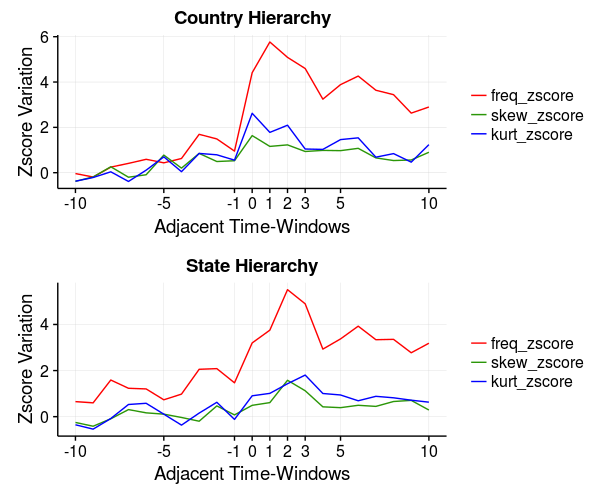
\includegraphics[width=\columnwidth]{img/labeled2.png}
	\caption{Average variation in emergency situations between time-windows.}
	\label{fig:labeled}
\end{figure}



\section{Experiments}

Our filtering task can be seen as binary classification task. The positive class (\textit{detection label}) corresponds to messages related to instantaneous emergency situations, while the negative class (\textit{nothing label}) corresponds to the remaining or non-related to crisis situations.

To classify messages we employed traditional binary classifier Support Vector Machine \textit{(SVM)}. As a result of the analysed data scattering (Figure \ref{fig:scatter}), we separated country and state in different datasets and set both kernels and classification parameters independentely. On the one hand, \textit{country} classifier uses a polynomial kernel and strict-parameters for gamma, cost and weights since a great amount of messages are included in country hierarchy as an effect of the minor hierarchies. On the other hand, \textit{state/region} classifier uses a linear kernel with soft-weights and cost.

\begin{figure}
	\centering
	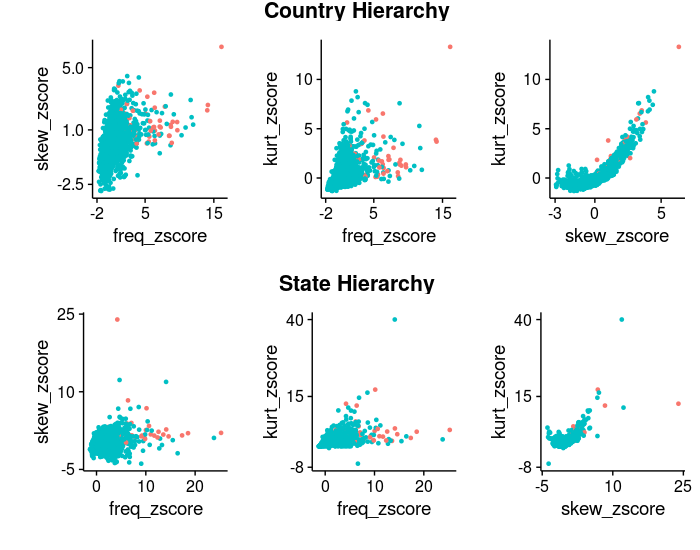
\includegraphics[width=\columnwidth]{img/scatter.png}
	\caption{Relationship between features in country and state hierarchy. Red circles represent positive class (\textit{detection}) and blue circles represent negative class (\textit{nothing}).}
	\label{fig:scatter}
\end{figure}


Given that an emergency situation is not an usual event, we have an highly unbalanced data respect to the classes after labeled ($1\approx2\%$ of positive class corresponding to \textit{detection}). Therefore, we used \textit{under-sampling} \cite{lunardon2014rose} over country and state datasets increasing our possitive class to $15\approx18\%$. Additionally, to validate our model, we used \textit{5-fold cross-validation} where one earthquake dataset is used as testing and the remaining earthquakes dataset as training.

Table \ref{tab:perfomance} shows the average results of our model applying 5-fold cross validation. In order provide a extended analysis about incorrect labels and time-windows, we include the metric \textit{False Positive Rate (FPR).} 


\subsubsection{Independent Analysis of Hierarchies} 
Our first analysis is just considering the hierarchies as isolated detections. The top of the Table \ref{tab:perfomance} shows the results considers only the prediction over each label in our datasets. As noted above, the assignation from the lowest level (\textit{city}) to the highest (\textit{country}) in the gazetteer hierarchy generated high frequency of messages which cause multiple \textit{bursts} in our country signal for non  emergency situations. This concept can explain the values of Precision (\textit{P}) and \textit{FPR}.

In addition to the analysis of number of detections by labels, we also study the number of detections by time-windows. For this analysis, we search the time-windows for each hierarchy where the all metadata-levels are well classified with correct class. According to the results shown on the middle of the Table \ref{tab:perfomance}, when we analyse country and state independentely the values of Precision, F1 and FPR have worst values than the analysis by label . 
\begin{table}
	\caption{Average performance of 5-fold cross-validation by hierarchy and geographic spread (G.S.)}.
	\label{tab:perfomance}
	\centering
	\begin{tabular}{c|lcccc}
		\toprule
		&Hierarchy &P &R &F1 &FPR\\
		\midrule
		\parbox[t]{2mm}{\vspace{-0.2cm}\multirow{3}{*}{\rotatebox[origin=c]{90}{\small{label}}}} 
		& Country & 0.3 & 0.83 & 0.45& 0.14\\		
		& State &0.35& 0.83& 0.5 & 0.08\\
		\midrule
		\parbox[t]{2mm}{\vspace{0cm}\multirow{5}{*}{\rotatebox[origin=c]{90}{\small{time-window}}}}
		& Country & 0.15& 0.77 & 0.25 & 0.15\\
		& State & 0.17 & 0.88 & 0.29& 0.12\\
		& Country-State& 0.35 & 0.7 & 0.47 & 0.03\\
		& Country(2)-State with G.S. & 1 & 0.64 & 0.78 & 0 \\
		& Country(3)-State with G.S. & 1 & 0.47 & 0.64 & 0\\
		\bottomrule
	\end{tabular}
\end{table}

\subsubsection{Dependent Analysis of Hierarchies}
Our second analysis considered the hierarchies as non-isolated detections. In the results explained above, we considered country and state hierarchy independently, which is not a correct analysis because an emergency situation affects states and country at the same time. For this reason, we inspected the time-windows where all metadata-level for country and state hierarchy have a correct detection simultaneously. The results are shown in the row \textit{Country-State} in the Table \ref{tab:perfomance}. In contrast to the independent analysis of country and state, we improved the Precision, F1 and FPR values as a consequence of a smaller amount of the time-windows related to non emergency situations are assigned as detection. However, when we see the value obtained for FPR ($FPR = 0.03$), this rate represents an incorrect number of time-windows assigned as detection equal to $23$. This means that we have $23$ new emergency situations detected by our classifier. 


\subsubsection{Geopraphic Spread Analysis}\label{sssec:geospreadanalysis}
Our third analysis considered the hierarchies as non-isolated detections and applies the Geographic Spread (G.S.). Using the \textit{Adjacency Matrix} to represent neighborhoods between regions/states, we considered as a correct detection those time-windows where the state/s classified as detection are defined as \textit{Focalized} or \textit{Diffused} and exist dependency between hierarchies. 

\begin{table*}
	\caption{Online evaluation by time-windows (T-W) using Country(2)-State with G.S. method}
	\label{tab:online1}
	\begin{tabular}{lccccp{3.5cm}c}
		\toprule
		Event &Detected T-W & T-W Before Event & T-W After Event & Delay (min) & Top 3 Bigrams\\
		\midrule
		Premier League Soccer Matches & 2& - & - & - & \small{(man, utd), (new, year), (happy, new)} \\
		Westminster Terrorist Attack& 13 & 0 &13 & 32& \small{(stay, safe), (terror, attack), (safe, everyone)}\\
		Manchester Terrorist Attack& 12& 1& 11& 23& \small{(ariana, grande), (incident, arena), (grande, concert)}\\
		London Terrorist Attack & 14 & 7 & 7 & 36 & \small{(stay, safe), (incident, bridge), (borough, market)}\\
		U.K. Elections& 5 & - & - & - & \small{(theresa, may), (vote, labour), (van, dijk)}\\
		Adele Live in Wembley& 9& 7&2&-& \small{(elland, road), (new, times), (phil, jackson)}\\
		England vs Slovenia Soccer Match & 4& 4 & 0 & - & \small{(simon, brodkin), (join, us), (theresa, may)}\\
		Metallica Live in London& 4 & 4 & 0 & - & \small{(always, said), (chance, win), (carabao, cup)}\\
		\bottomrule
	\end{tabular}
\end{table*}


\begin{table*}
	\caption{Online evaluation by time-windows (T-W) using Country(3)-State with G.S. method}
	\label{tab:online2}
	\begin{tabular}{lccccp{3.5cm}c}
		\toprule
		Event &Detected T-W & T-W Before Event & T-W After Event & Delay (min) & Top 3 Bigrams\\
		\midrule
		Premier League Soccer Matches & 0& - & - & - & \hfill \break \\
		Westminster Terrorist Attack& 4 & 0 &4 & 32& \small{(terror, attack), (stay, safe), (terrorist, attack)}\\
		Manchester Terrorist Attack& 2& 0& 2& 23& \small{(ariana, grande), (praying, everyone), (everyone, affected)}\\
		London Terrorist Attack & 1 & 1 & 0 & - & \small{(ariana, grande), (around, world), (lady, gaga)} \\
		U.K. Elections& 0 & - & - & - & \hfill \break\\
		Adele Live in Wembley& 0& 0&0&-& \hfill \break\\
		England vs Slovenia Soccer Match & 1& 1 & 0 & - & \small{(per, day), (menswear, sample), (closed, roads)}\\
		Metallica Live in London& 2 & 2 & 0 & - & \small{(happy, birthday), (chance, win), (always, said)}\\
		\bottomrule
	\end{tabular}
\end{table*}


In addition to the results of the dependency analysis explained above, we see that a large amount of time-windows for country hierarchy ($\approx 82\%$) have more than one metadata-level when exist a correct detection. This can be explained since an emergency situation produce a collective reaction on the level of body of the message (\textit{tweet text}), users sharing any messages with profile location in a specific country (\textit{user location}) or mixing both concepts (\textit{tweet text - user location}).


Considering the geographic spread by states and the number of metadata-levels by country hierarchy, we analysed the results shown on the bottom of the Table \ref{tab:perfomance}. On the one hand, the row with value equal to \textit{Country(2)-State with G.S.} represents the detection when we considered at least two metadata-levels for the country hierarchy and the geographic spread for states. In contrast to the the previous analyses, we improved the values of the Precision, F1 and FPR. The last metrics are very important because there are no time-windows incorrectly assigned as emergency situations. Consequently, the Recall values decrease which means that our method remove some time-windows classified as detection. Beside the percent of emergency situations detected is equal to $100\%$ with a average delay equal to $10.4$ minutes ($min=6$, $max=14$) from the impact of the event to the first detection.


On the other hand, \textit{Country(3)-State with G.S.} represent the detection when we considered three metadata-levels for country hierarchy and the geographic spread for states. Similar to  \textit{Country(2)-State with G.S.}, we improved the values of Precision, F1 and FPR but our recall decrease from $R = 0.58$ to $R = 0.47$, detecting  $80\%$ of the emergency situations with a average delay equal to $11.5$ minutes ($min=8$, $max=14$) from the impact of the event to the first detection.




\subsection{Online Evaluation}
For our evaluation in the Twitter Public Stream, we trained classifier with five earthquakes identified in our ground truth. Furthermore, our evaluation dataset is formed by eight different events that occurred in England between December 2016 and October 2017. For each event we considered the full-day in which they ocurred. The main goals of this evaluation is to know the capacity of our method to detect emergency situations and discard those non-related to emergency events that involve location references. Geographic spread analysis is used to evaluate our method because decrease the number of false positives detection. In the same way of the experiments in Section \ref{sssec:geospreadanalysis}, we compare the results using the two presented methods respect to the number of metadata-levels by country hierarchy.

As can be noted on Table \ref{tab:online1} and Table \ref{tab:online2}, we study three terrorist attacks and five high-impact real-world events related to soccer matches, music concerts and political elections. In the case of Premier League Soccer Matches and U.K Elections, we can not identify the beginning of the event, since in the first one there are many soccer matches during the analysed day and in the second one there is no a specific start time. In order to know the topics when our method detects an event, we computed the Top 3 Bigrams in the detected time-windows. Also, we calculated the delay time just for emergency events.

On the one hand, the first evaluation \textit{Country(2)-State with G.S.} has full detection of the terrorist attacks with average delay time equal to $30.3$ minutes. These detections are related to the event given that the bigrams represent terms associated with crisis situations. However, the London Terrorist Attack has $50\%$ of the detected time-windows after the event, which means that there are seven time-windows non-related to emergency situations. Besides the crisis situations analysis, we also study the number of detected time-windows in non-related to emergency situation events. In the same way, we have a large amount of misclassified time-windows that do not represent crisis situations as we can see in the Top 3 Bigrams for each non-related to event.



On the other hand, the second evaluation \textit{Country(3)-State with G.S.} decreases the number non-related to emergency situations events detected as crisis situations. We can see three time-windows in two events detected as emergency situations (England vs Eslovenia, and Metallica Live in London). In these cases, the time-windows are detected before the event and corresponding a non emergency situations according to the bigrams. Furthermore, when we analysed the number of the detected emergency situations, two-thirds ($66\%$) of the events are detected correctly with average delay time equal to $30.3$ minutes. In the case of London Terrorist Attack, our method detects one time-window before the event but the bigrams describe that the detections do not correspond to crisis situations.

%Unlike to  \textit{Country(2)-State with G.S} method, \textit{Country(3)-State with G.S} method decreases the number of detection by time-windows given that latter is stricter than the first one respect to the number of country detection by metadata-level.


\begin{figure}
	\centering
	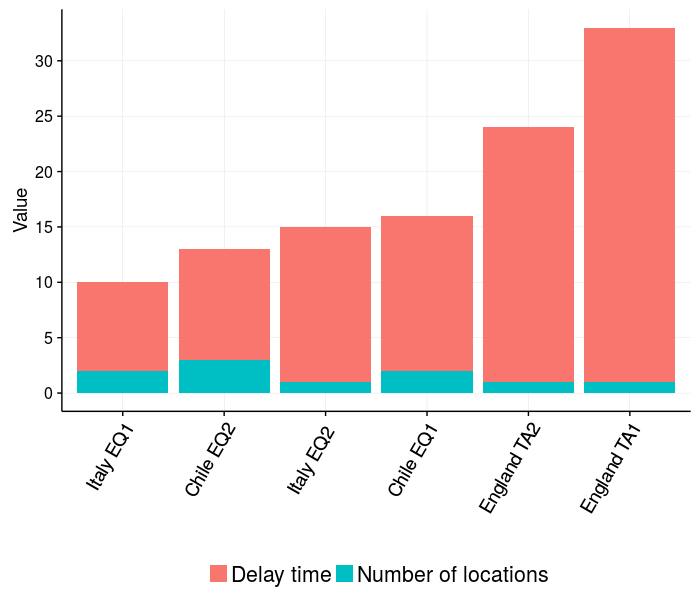
\includegraphics[width=\columnwidth]{img/delay.png}
	\caption{Delay time and number of locations in the first detection for diffused and focalized emergency situations.}
	\label{fig:delay}
\end{figure}

\section{Discussion}

Our findings suggest that there is evidence to detect an emergency situation based on anomaly frequency of messages that contain locations for a specific country. Indeed, our method based on the number of metadata-levels by country hierarchy and geographic spread by state, detects a $80\%$ of the events related to emergency situations as we could demonstrate in our ground truth. Also, our method is independent of the textual features because we apply the model over different languages as Spanish, Italian and English. Furthermore, we test our model in different types of events such as earthquakes and terrorist attacks, and also on different magnitudes (in the case of earthquakes) and number of affected people (e.g., Manchester Terrorist Attack vs Westminster Terrorist Attack).

However, when we apply our method in the on-line evaluation, we detect $66\%$ of the emergency situations that affected England. This explains that the signals, and for various reasons: the number of active users in United Kingdom\footnote{http://www.statista.com/statistics/242606/number-of-active-twitter-users-in-selected-countries/ visited on January 2018} which can affect the anomaly frequency of the messages since there exists a high daily average activity of the messages; similar locations in other countries (York $\approx$ New York); and soccer teams with names of cities (Manchester United, Liverpool). These issues also can affect the number of false positive detection in which in the case of England was $30\%$ of the non-related to emergency events.

Regarding the geographic spread where we define an emergency situation as diffused or focalized, we find some evidence that differentiates them. In the case of diffused events, the delay time of the our first detection was less than $12$ minutes and in focalized events was greater than $30$ minutes (Figure \ref{fig:delay}). This explains that, in diffused events such as earthquakes, a high number of people are affected (thousands or millions) at the same time by an event which generates a collective reaction in social media in the locations where the event impacted. In Figure \ref{fig:delay}, we can see that earthquakes have at least two detected locations in the first detection (except Italy EQ2). In contrast, focalized events have less amount of eyewitness (hundreds or thousands) then when the users share messages in social media, the frequency does not affect the average daily message of the country in the first minutes. This can be explained in Figure \ref{fig:delay} where the terrorist attacks have just 1 detected location in the first detection.

Additionally, the delay time can be different for many reasons: datetime of the event (for example, during the early hours), few differences with the end of the current time-window, type of the affected locations (rural, urban cities) and the number of active users by locations.

%\begin{itemize}
%	\item explain that we dont need compute textual features as bigrams, top-k terms.
%	\item explain that we just need de gazetteer tree
%	\item explain when our methodology could be not working. eg. why not working correctly in england. country with many language. How event like soccer match are filtered and when not working
%	\item Delay time: explain difference between focalized and diffused event. People feel the event at the same time, activity in affected locations.
%	\item Number of locations affected in the first and second detection for focalized and diffused (plot)
%	\item Diffused: mercalli and locations detected.
	
%\end{itemize}

\section{Conclusion}

In this paper we have presented a methodology for detecting an emergency situation based on location for a specific country. This approach is independent of the textual features and can be used in different types of events and languages. We show that the users act as self-organized in the affected locations like citizen sensors when an emergency situation occurs. We furthermore have presented an analysis of geographic spread for different types of events that can be categorized. However, our experiment considers just a small portion of emergency situations, which is not representative for all types of crisis situations according to either the hazard type (natural or human-induced), temporal development (instantaneous or progressive) or geographic spread (diffused or focalized).

There are many things that can improve our results. We will add Point of Interest to our gazetteer tree to increase the frequency by time-windows in each hierarchy. Furthermore, we will add more non-textual features as number of retweets and tweets, unique locations detected and special locations. We also plan to study the relevance of the different metadata-levels and assign weights for each. Finally, we will create a web application to visualize events in real-time.

%\begin{acks}
	
%\end{acks}



\bibliographystyle{ACM-Reference-Format}
\bibliography{bio} 

\end{document}
